\documentclass[11pt]{article}
\usepackage{jas_packages}
\usepackage{fix-cm}
\usepackage{jas_tikz_packages}
% custom macros for AAS paper
% Poincar\'e correct name
\newcommand{\Poincare}{Poincar\'e }

% Bold face for vectors 
\renewcommand{\vec}[1]{\mathbf{#1}} % vec command now makes it boldface
\let\oldhat\hat
\renewcommand{\hat}[1]{\oldhat{\mathbf{#1}}} % using a hat also makes it boldface

% Macros for discrete states to save some time typing
\newcommand{\xk}{\ensuremath{x_k}}
\newcommand{\xkp}{\ensuremath{x_{k+1}}}
\newcommand{\yk}{\ensuremath{y_{k}}}
\newcommand{\ykp}{\ensuremath{y_{k+1}}}

\newcommand{\pxk}{\ensuremath{p_{x_k}}}
\newcommand{\pxkp}{\ensuremath{p_{x_{k+1}}}}
\newcommand{\pyk}{\ensuremath{p_{y_k}}}
\newcommand{\pykp}{\ensuremath{p_{y_{k+1}}}}

\newcommand{\xdotk}{\ensuremath{\dot{x}_{k}}}
\newcommand{\ydotk}{\ensuremath{\dot{x}_{k}}}
\newcommand{\xdotkp}{\ensuremath{\dot{x}_{k+1}}}
\newcommand{\ydotkp}{\ensuremath{\dot{y}_{k+1}}}

\newcommand{\distonek}{\ensuremath{r_{1_k}}}
\newcommand{\distonekp}{\ensuremath{r_{1_{k+1}}}}
\newcommand{\disttwok}{\ensuremath{r_{2_{k}}}}
\newcommand{\disttwokp}{\ensuremath{r_{2_{k+1}}}}

% costate equations of motion (gauss jordan elimination)
\newcommand{\fonex}{\ensuremath{f_{1_x}}}
\newcommand{\ftwox}{\ensuremath{f_{2_x}}}
\newcommand{\fthreex}{\ensuremath{f_{3_x}}}
\newcommand{\ffourx}{\ensuremath{f_{4_x}}}

\newcommand{\foney}{\ensuremath{f_{1_y}}}
\newcommand{\ftwoy}{\ensuremath{f_{2_y}}}
\newcommand{\fthreey}{\ensuremath{f_{3_y}}}
\newcommand{\ffoury}{\ensuremath{f_{4_y}}}

\newcommand{\fonexd}{\ensuremath{f_{1_{\dot x}}}}
\newcommand{\ftwoxd}{\ensuremath{f_{2_{\dot x}}}}
\newcommand{\fthreexd}{\ensuremath{f_{3_{\dot x}}}}
\newcommand{\ffourxd}{\ensuremath{f_{4_{\dot x}}}}

\newcommand{\foneyd}{\ensuremath{f_{1_{\dot y}}}}
\newcommand{\ftwoyd}{\ensuremath{f_{2_{\dot y}}}}
\newcommand{\fthreeyd}{\ensuremath{f_{3_{\dot y}}}}
\newcommand{\ffouryd}{\ensuremath{f_{4_{\dot y}}}}
\usepackage[letterpaper,margin=1in,centering]{geometry}
\usepackage{graphicx}
\usepackage{amssymb}  
\usepackage{amsmath}
\usepackage{amsfonts}
\usepackage{siunitx}
\usepackage{mathtools}
\usepackage{microtype}
\usepackage{color}
\usepackage{bm}
\usepackage{xr-hyper}
% \usepackage{nameref,zref-xr}
\usepackage{hyperref}
\usepackage[]{cleveref} % get fancy referencing

% \zexternaldocument{manuscript}
\externaldocument[]{manuscript}[manuscript.pdf]

% edit cref citations for IEEE format
\crefformat{equation}{(#2#1#3)} % no abbreviation for equation numbers
\Crefformat{equation}{Equation~(#2#1#3)} % no abbreviation for equation numbers
\crefrangeformat{equation}{(#3#1#4--#5#2#6)}
\Crefrangeformat{equation}{(#3#1#4--#5#2#6)}
\crefmultiformat{equation}{(#2#1#3)}{ and~(#2#1#3)}{, (#2#1#3)}{ and~(#2#1#3)}
% edit cref citations for IEEE format
\crefformat{figure}{Fig.~#2#1#3} % no abbreviation for equation numbers
\Crefformat{figure}{Fig.~#2#1#3} % no abbreviation for equation numbers
\crefrangeformat{figure}{Figs.~#3#1#4--#5#2#6}
\Crefrangeformat{figure}{Figs.~#3#1#4--#5#2#6}
\crefmultiformat{figure}{Figs.~#2#1#3}{ and~#2#1#3}{, #2#1#3}{ and~#2#1#3}
% for items in a list
\crefformat{enumi}{(#2#1#3)}
\Crefformat{enumi}{Item~(#2#1#3)} 
\crefrangeformat{enumi}{(#3#1#4--#5#2#6)}
\Crefrangeformat{enumi}{Items~(#3#1#4--#5#2#6)}
\crefmultiformat{enumi}{(#2#1#3)}{ and~(#2#1#3)}{, (#2#1#3)}{ and~(#2#1#3)}
% Proposition format
\crefformat{prop}{Proposition~#2#1#3} % no abbreviation for equation numbers
\Crefformat{prop}{Proposition~#2#1#3} % no abbreviation for equation numbers
\crefrangeformat{prop}{Proposition~#3#1#4--#5#2#6}
\Crefrangeformat{prop}{Propositions~#3#1#4--#5#2#6}
\crefmultiformat{prop}{Propositions~#2#1#3}{ and~#2#1#3}{, #2#1#3}{ and~#2#1#3}
% Appendix
\crefformat{appendix}{Appendix~#2#1#3} % no abbreviation for equation numbers
\Crefformat{appendix}{Appendix~#2#1#3} % no abbreviation for equation numbers
\crefrangeformat{appendix}{Appendices~#3#1#4--#5#2#6}
\Crefrangeformat{appendix}{Appendices~#3#1#4--#5#2#6}
\crefmultiformat{appendix}{Appendices~#2#1#3}{ and~#2#1#3}{, #2#1#3}{ and~#2#1#3}

\newcommand{\RNum}[1]{\uppercase\expandafter{\romannumeral #1\relax}}
\newcommand{\RI}{\text{\RNum{1}}}
\newcommand{\RII}{\text{\RNum{2}}}
\newcommand{\RIII}{\text{\RNum{3}}}

\newtheorem{definition}{Definition}
\newtheorem{lem}{Lemma}
\newtheorem{prop}{Proposition}
\newtheorem{cor}{Corollary}

\newenvironment{correction}{\begin{list}{}{\setlength{\leftmargin}{1cm}\setlength{\rightmargin}{1cm}}\vspace{\parsep}\item[]``}{''\end{list}}

\begin{document}

%\pagestyle{empty}

\section*{Response to the Reviewers' Comments for JASS-D-17-00005}

I would like to thank the reviewers for their thoughtful comments, which are aimed towards improving the quality of the manuscript and the clarity of the results. 
In accordance with the comments and suggestions, the manuscript has been revised, and the answers to all comments are addressed as follows.

(In the revised manuscript, the citation numbers for equations, assumptions, propositions, and references are changed. This answer is written according to the new item numbers.)

\subsection*{Reviewer 1} 
\begin{itshape}
Reviewer \#1: I have some issues with this paper that, in my opinion necessitate a major revision.
These issues are:
\end{itshape}

\begin{itemize}
    \item 
        \begin{itshape}
-It extensively re-covers issues that have been covered in many papers, making it difficult to disseminate what the original contributions are.  For example, I don't think the addition of the thrust term into the dynamics necessitates re-doing every piece of analysis that has been done with various resources in the literature about variational integrators (including comparisons with RK methods).  Things that can be found in other research should be cited, and summary comments can be used to point the readers to fill in this knowledge.  The content of this paper easily be reduced considerably to maintain focus on the original contributions.
    \end{itshape}

    The paper is being reduced. 
    The introduction has been reduced to avoid excessive repetition. 
    In addition, much of the background material has been removed

\item
    \begin{itshape}
-It does not give a complete picture of the pros and cons of the proposed methodology.  This method is full of both advantages and disadvantages.  I don't think the authors need to be concerned with "selling" the work to the community, but rather showing the full and honest picture given the current state of the research.  In the conclusions, the potential cons to this research can be mitigated by setting a path forward for future research to further improve the methodology.

These pros/cons include:

-The formulation of the problem with acceleration magnitude is a major technical challenge for mission design practitioners.  The state of the art to design trajectories that depend on low-thrust engine hardware is either:

-To produce constant thrust magnitude or no thrust magnitude (typical of nuclear electric propulsion, or very simple electric propulsion systems.)

-To produce variable thrust magnitude associated with various throttle points at different power accessibility levels (solar electric propulsion).
That is not to say that useful solutions cannot be extracted from the problem, as the authors have shown.  However, a great many solutions in this approach will be unusable due to the fact that acceleration and thrust magnitude are different, i.e. a=T/m

Thus - a MAJOR focus of future work should be the introduction of a seventh state (mass).  This gives rise to a more challenging optimal control problem requiring the switching function, but it is the form that is generally needed in computing optimal open-loop trajectories that can actually be flown.
\end{itshape}

\item 
    \begin{itshape}
The pros and cons of the PCRTBP

-The PCRTB gives rise to exploiting Poincare sections in a systematic manner.  2D solutions might be close enough for qualitative understanding of the solution space for many problems (as long as large plane changes aren't needed).

-The PCRTB is limiting for many pragmatic departure orbits (e.g. LEO and GTO, the most common departure orbits for low-thrust transfers).
\end{itshape}

Additional detail has been included in the problem formulation section.
This includes some discussion on the choice of the PCRTBP and the relative strengths/weaknesses of this approach.
The additional paragraph has been copied below.

\begin{correction}
We utilize the planar circular restricted three body problem~(PCRTBP) as the basis of our system definition. 
It is a popular model in the preliminary analysis of multibody spacecraft trajectories. 
In the context of Earth based mission, the PCRTBP affords a relatively simple dynamic model while still capturing the major third body perturbation of the Moon.
In addition, this model allows for a systematic process to define and exploit \Poincare sections.
Furthermore, the 2D solutions afforded by the PCRTBP are frequently use to gain a qualitative understanding of the trade space of transfers in the Earth-Moon system.
The PCRTBP approach offers insight into the fundamental dynamical structure while capturing the major dynamic properties of the planar motion.
As a result, this approach is best suited for trajectories which do not require large plane changes.
\end{correction}

\item 
    \begin{itshape}
The pros and cons of variational integrators should really be acknowledged rather than completely dismissing the RK methods which are still the current state of the art in mission design (using higher-orders and suitable tolerances)

-Pros = boundedness in the energy behavior.  Very long term integration will not deviate from the known dynamical structure.

-Cons = you don't know where you are on the energy surface, just that you are on it somewhere.  This is still a problem in actual trajectory design.  Knowing the error is on an energy surface does not mean that you don't have error.
\end{itshape}
\end{itemize}
From here on out comments specific to various sections of the paper follow:

\begin{enumerate}
    \item
        \begin{itshape}
            In the statement "In addition, non-Keplerian orbits and multi-body dynamics have been shown to allow for a much greater range of potential
            missions at a reduced energy cost [15]" - you may want to reference, for example, the Lunar Ice Cube mission paper which absolutely requires low-thrust propulsion and non-keplerian dynamics to satisfy its mission objectives.

            Folta, D., Dichmann, D., Clark, P., Haapala, A., and Howell, K., "LunarCube Transfer Trajectory Options," AAS/AIAA Space Flight Mechanics Meeting, Williamsburg, Virginia, January 11-15, 2015.
        \end{itshape}

        The introductory paragraphs have been reworded and reorganized for clarity. 
        Specifically, the first paragraph has been divided, which motivates the use of electric propulsion and the advantages of small satellites which use electric propulsion.
        In addition, the suggested reference has been included in the paper.
        The modified paragraphs are duplicated below.

        \begin{correction}
            Designing spacecraft trajectories is a classic and ongoing topic of research.
            There has been significant research into the design of orbital transfers for space vehicles.
            Optimal expenditure of onboard propellant is critical to allowing a mission to continue for a longer period of time or to enable the launch of a less massive spacecraft.
            Electric propulsion systems offer a much greater specific impulse than chemical systems.
            As a result, the greatly increased effeciency allows for greater payload mass or extended duration missions.
            However, these electric propulsion systems typically have much less thrust than their chemical counterparts and therefore orbital manuevers have a much longer time of flight.
            In spite of this drawback, a wide variety of missions, such as communication and deep space probes, have utilized the unique benefits of low thrust electric propulsion to great effect~\cite{choueiri2009}.

            With reduced development intervals and decreased launch costs, small satellites have gained increased attention as a cost effective means of scientific and technologic development. 
            Furthermore, these cubesats are easily launched as secondary payloads rather than requiring a dedicated launch.
            The merger of small satellites with miniature electric propulsion enables inexpensive and responsive missions requiring large changes in orbital energy or extended mission lifespan.
            Recent developments in miniature electric propulsion offer the potential for new research opportunities for small spacecraft~\cite{haque2013}.
            The advancements in minature electric propulsion allows for greater flexibility in the deployment of cubesats as secondary payloads.
            Without the explicit requirement of a dedicated launch trajectory, cubesats are able to exploit a much wider range of possible mission designs~\cite{folta2015}.
            With the potential for more demanding missions, even greater importance is placed on the mission design to ensure that optimal trajectories satisfy mission requirements. 
            In addition, non-Keplerian orbits and multi-body dynamics have been shown to allow for a much greater range of potential missions at a reduced energy cost~\cite{folta2015,koon2011}.
            Future space missions are increasing in complexity and will require new classes of orbits that are not possible via the traditional patched-conic approach~\cite{ross2006,gomez2001}.
            Optimally combining the structure of the dynamic environment with low-thrust propulsion systems is vital for future mission success.
        \end{correction}

\item 
    \begin{itshape}
"Since there is an insufficient number of analytical constants, or integral of motion, numerical methods must be used to investigate solutions to the three-body problem."  This isn't completely true as there are also approximations to the (uncontrolled) three-body motion, such such as the Richardson-Cary approximation.  Saying numerical methods are required may be a bit strong.  May want to say "often required".
\end{itshape}

The sentence has been modified as follows.

\begin{correction}

Finally, there is no closed form analytical solution for the three-body problem and there are an insufficient number of analytical constants~\cite{szebehely1967}.
As a result numerical methods are often required to investigate solutions to the three body problem.
\end{correction}

\item 
    \begin{itshape}
"These techniques suffer from numerical instability and energy drift behaviors which make them ill-suited for long-term propagation. These dissipative effects are even more detrimental with the addition of low-thrust propulsion to the dynamic equations of motion."  It really depends on what you mean by "long term".  If transfers are on the order of hundreds of days, then high precision runge-kutte integrator, for example a Runge-Kutte Verner 8(9), can maintain suitable accuracy such that the energy drift in the Hamiltonian is very small, as can be seen in some of the references that the authors have cited.  If, on the other hand you mean 10-100's of years or more, i.e., when you create your Poincare maps, then this drift is more apparent.  I think that this statement needs to be quantified better because it gives a dishonest portrayal of high-precision Runge-Kutte integrators without numbers attached to it.
\end{itshape}

\item
    \begin{itshape}
"Conventional integration techniques fail to capture the physical laws and geometric properties of the dynamic system [8]. As a result, the long term effects of low-thrust on the spacecraft trajectory are not accurately captured."  Again, I think situationally I would disagree.  Transfers on the order of 100's of days can maintain accuracies of 1e-10 (nondimensional units) in the Hamiltonian, which is generally considered a "small" amount of energy drift.
\end{itshape}

These sentences have been modified and combined to enhance clarity and reduce some of the unecessary bloat. 
In addition, some additional detail has been added to explicitly define the notion of ``long-term'' in the context of numerical integration.
The modifications are copied below.
\begin{correction}
    Conventional Runge-Kutta integration techniques, such as those implemented in~\cite{mingotti2011,grebow2011}, fail to capture the physical laws and geometric properties of the dynamic system.
    As a result, these methods suffer from numerical instability and energy drift behaviors which make them ill-suited for the long-term propagation, e.g. on the order of decades to centuries, which is typical of the three-body problem. 
\end{correction}

\item 
\begin{itshape}
- "[15,25] have illustrated the rich structure that exists in the three-body problem." 
- "[23,6] implement the solutions using conventional Runge-Kutta integration techniques."
I don't think you can grammatically begin a sentence with reference numbers.  Please fix all instances of this.
\end{itshape}

The sentences have been reworded to avoid starting with a reference number. 
The corrections are shown below.

\begin{correction}
    \begin{itemize}
        \item Conventional Runge-Kutta integration techniques, such as those implemented in~\cite{mingotti2011,grebow2011}, fail to capture the physical laws and geometric properties of the dynamic system.
        \item There exists a rich structure in the three-body problem~\cite{koon2011,ross2006}.
    \end{itemize}
\end{correction}

\item 
    \begin{itshape}
"It has been shown that there exist multi-dimensional tubes, or invariant manifolds, of constant energy trajectories that span the state space."  The "tube" statement is really only true for some libration point orbits at certain Jacobi Constants.  For some orbits these structures are more chaotic and don't resemble tubes.  May want to soften this language or change "tubes" to "structures".
\end{itshape}

The sentence has been modified as follows.

\begin{correction}
It has been shown that there exist multi-dimensional structures, termed invariant manifolds, of constant energy trajectories that span the state space. 
\end{correction}

\item 
    \begin{itshape}
-"In this paper, we propose a systematic design method which enables low-thrust transfers in the planar circular restricted three-body problem." Why planar?  For simplicity?  Almost all parking orbits departing the Earth are likely going to have some inclination with respect to the rotating reference plane, and will likely require some three-dimensional thrusting to target the manifold.  You may want to indicate that this is a first step in the research to exploit the Poincare sections more easily, which is why I'm assuming it was done.  It doesn't hurt to be straightforward about this, as it is a first-step towards characterizing the design space.
\end{itshape}

The introduction has been modified with an additional sentence indicating our use of the planar three body problem

\begin{correction}
Utilizing the planar assumption greatly simplifies the problem and allows for the use of established methods in determining periodic orbits and \Poincare sections.
\end{correction}

\item 
    \begin{itshape}
-"In addition, through the use of geometric integrators we accurately capture the effects of low thrust on the system dynamics in the numerical simulation."  A variational integrator will accurately capture the qualitative effects of the transfer (e.g. propellant use), however it will not necessarily accurately capture accuracy in the final state vector - it is guaranteed to be on an energy surface, but it is not guaranteed to be at exactly the right location on the energy surface.  I would soften this claim or reword.
\end{itshape}

While the geometric integrator will not exactly characterize the terminal energy or state of a dynamic system, it will better preserve the total energy variation as compared to convential integration schemes. 
In addition, the total energy deviation will remain bounded and less than than of convential schemes which experience unbounded energy deviation. 
As a result, the terminal state/energy will be more accurately characterized using a variational integrator as compared to conventional schemes. 
Also this difference becomes more evident over increasing time horizons.
Some additional detail has been added stating that the increased accuracy is most evident over long time periods. 

\begin{correction}
In addition, through the use of geometric integrators we more accurately capture the effects of low thrust on the system dynamics in the numerical simulation over extended periods which are typical of electric propulsion systems. 
\end{correction}

\item 
    \begin{itshape}
-"The Poincare section reduces the dimensionality of the system dyanmics to the study of a related discrete update map." It does, but at the expense if a large up-front computational run that must be run well in advance to capture the problem characteristics.  Also, it is more challenging to execute in 3D, which should be noted.
\end{itshape}

Some additional detail has been included mentioning the difficulties in applying the \Poincare~section approach to the 3D case.

\begin{correction}
While the \Poincare~section is well defined for the planar case, as a 2D representation, it is more challenging to implement and visualize for the general 3D three-body problem.
\end{correction}

\item
    \begin{itshape}
-"This discrete update map, or variational integrator, shares the same geometric properties of the continuous time system and exhibits much better energy behavior than the traditional integration methods, especially over long transfer durations with small magnitude control inputs."  Yes, but the order of the variational integrator still matters.  The drift in the state vector accuracy is still important to a mission designer, even if it is guaranteed to lie on an energy surface.  I think you should indicate that this is more for preliminary analysis to characterize the transfers, when this drift in state vector accuracy is tolerable.  I.E., it's useful for the introductory phases of mission design when trying to globally characterize the design space.  Characterizing the scope of the analysis in this way would be helpful to the audience.
\end{itshape}

The section on the variational integrator has been reduced and this specific sentence has been removed. 
However, additional detail has been provided in a different section of the paper which discusses this drawback of the variational integrator.

\begin{correction}
Over long simulation horizons or with the addition of small control inputs the inability of conventional integration schemes to accurately track the system energy limits the applicability of conventional techniques in which energy conservation is mandatory for characterizing the solution space.
In spite of this improved energy behavior, the order and design of the variational integrator still play an important role in the accuracy of the state vector.
This work uses a second order integrator which has improved energy behavior but potentially lower state accuracy as compared to high order Runge Kutta methods. 
However, for this preliminary analysis the variational integrator provides reduced computational demands and is useful to characterize and explore the trade space in preliminary mission design scenarios.
\end{correction}
\item 
    \begin{itshape}
"Optimal solutions are generally sensitive to small variations in the initial multipliers. As a result, the numerical stability of sensitivity derivatives is critical to accuracy and computational performance."  I don't agree that this implies that variational integrators are better for gradient-based methods.  The primary issue is that gradient-based methods that are solving optimal control problems are using first-order approximations to iterate on the problem.  The first-order approximation is what is poor, not necessarily the gradients.  Even if these gradients are of exact accuracy (and I agree that they should always be as accurate as possible), the first-order methods in the chaotic problem are what give the difficulties.  One could use a variational or standard integrator in a first-order gradient based method and nothing will change the fact that the method will be highly sensitive, save for partitioning the sensitivities as you did with your multiple shooting approach.  At best, you can change the statement to indicate that the accuracy in the gradients may improve, which is always helpful to gradient-based methods, but it's no guarantee that it eliminates major problem sensitivity.
\end{itshape}

This sentence has been removed from the introduction.
However, this is a valid comment and is noted for the future.

\item
    \begin{itshape}
Authors may also want to point out the loss of accuracy in variable step integrators that can also degrade first-order gradient based methods.  I didn't see this anywhere and it's something that should be acknowledged.  Basically, variable step integrators will introduce artificial "noise" into the gradients:

Pellegrini, E.P., Russell, R.P., On the Accuracy of Trajectory State Transition Matrices, Paper AAS-15-785, AAS/AIAA Astrodynamics Specialist Conference, Vail, CO, Aug 2015
\end{itshape}

\item 
    \begin{itshape}
"This results in an optimal solution rather than the suboptimal solution typical of direct optimal control methods." I disagree that suboptimality is typical of direct methods.  A direct method will typically solve the KKT conditions, which can be directly transcribed into the costates in the optimal control problem.  A direct method fully satisfying the KKT conditions can map to the indirect problem. If you want to strengthen this argument, then you should argue that it applies to direct methods which rely on coarse or suboptimal representations of the control.  For example, a hybrid direct method could use continuous optimal control theory control law, but directly minimize the cost function instead of solving the full TPBVP.  
\end{itshape}

\item 
    \begin{itshape}
"Application of the Euler-Lagrange equations results in following equations of motion defined in the rotating reference frame"  Add a reference after this statement for those who want to see the derivation.  One of the given references probably does already does this, so just pick one
\end{itshape}

An additional comment has been included in the problem formulation section with a reference to a source of the detailed derivation.
\begin{correction}
Following a straightforward application of the Euler-Lagrange equations, a more detailed derivation is provided in~\cite{szebehely1967}, results in the following equations of motion defined in the rotating reference frame
\end{correction}

\item 
    \begin{itshape}
It appears from equation 5 and your control input definition that you control is unbounded?  Later on in reading the paper I found that you do add bounds on the control.  You may want to indicate earlier on in the paper (closer to eq. 5) that bounds will be added to the control.
\end{itshape}

An additional comment has been included mentioning that the control is assumed to be bounded in magnitude.

\begin{correction}
\ldots and the control inputs is defined as \( \vecbf{u} = \begin{bmatrix} u_x & u_y \end{bmatrix}^T \in \R^{2\times1} \) and assumed to be continuously variable but bounded in magnitude, i.e. \( \vecbf{u}^T \vecbf{u} \leq u_{max}^2 \).
\end{correction}

\item 
    \begin{itshape}
Figure 1 should probably have "axis equal" applied to it.  For that matter, please check all trajectory plots (those which plot the position state), and ensure that all plots are using "axis equal".  If not, please regenerate those plots. 
\end{itshape}

All of the figures showing position states have been modified to use \texttt{axis equal}.

\item 
    \begin{itshape}
Section 3.1 has been discussed in many references, the reader may want to direct them to this material.
(Choose one of Marsden or West's papers for example.)
\end{itshape}

The discussion on the variational integrators has been reduced. 
Much of the background material on Lagrangian mechanics is removed and an additional paragraph is included to summarize the key ideas of variational integrators. 
The additional paragraph is shown below.

\begin{correction}
Geometric numerical integration deals with numerical integration methods which preserve the geometric properties of the flow of a differential equation, such as invaraint properties and symplecticity.
Variational integrators are constructed by discretizing Hamilton's principle rather than the continuous Euler-Lagrange equations.
As a result, integrators developed in this manner have the desirable properties that they are symplectic and momentum preserving.
In addition, they exhibit improved energy behavior over long integration periods.
A thorough discussion of variational integrators is provided in~\cite{west2004,marsden2001}.
We use this approach to construct a variational integrator for the PCRTBP with the inclusion of low-thrust propulsion.

Consider the autonomous mechanical system described by the Lagrangian, \( L(q, \dot{q} ) \), for the generalized coordinates, \( q\) and velocities \( \dot{q} \).
The integration of the continuous Lagrangian along a path, \( q (t) \), followed by the system must satisfy Hamilton's principle, which results in the well-known Euler-Lagrange equations~\cite{lanczos1970}.
In the discrete time scenario, the continuous path \( q(t), \dot{q}(t) \), is replaced by a finite difference approximation over a fixed time step, e.g. \( q_0, \frac{q_1 - q_0}{h} \), which converges to the true velocity as \( h \) tends towards zero.
In this manner, we define a discrete Lagrangian, \( L_d (q_0, q_1, h) \) which approximates the integral of the true Lagrangian over the time interval \( h \) between \( q_0 \) and \( q_1\)~\cite{marsden2001}.
\end{correction}

\item 
    \begin{itshape}
The second-order trapezoidal rule will give significantly poorer state vector accuracy with respect to a high-precision RK integrator, even if the state is guaranteed to lie on an energy surface.  Why didn't the authors consider going to a higher-order variational integrator, or even a Taylor Integrator?  It is very likely that the integration accuracy will introduce some errors in the accuracy of the partial derivatives and in the states.
\end{itshape}

We chose the trapezoidal rule as it provides a second order quadrature approximation.
In addition, it provides an explicit rule that eases the complexity in using an implicit solution method.

\item 
    \begin{itshape}
Section 3.2 - please cite a reference as to where the selected quadrature rules presented in Table 1 have been derived.
\end{itshape}

In the interest of conciseness and to avoid repeating material that has already been covered in the literature, the discussion on variational integrators has been substantially reduced.
As a result, this table has been removed from the manuscript.

\item 
    \begin{itshape}
Figure 2 - x-axis has no label but I think it's nondimensional time, please indicate.  Label all axes even if they are nondimensional units.
\end{itshape}

The plot has been removed and replaced with another comparision between the variational integrator and \texttt{ODE45}.
In addition, all of the plots now have axis labels.

\item 
    \begin{itshape}
I recommend removing appendix B.  Giving the equations and stating that the Matrix inversion is from Gauss-Jordan elimination is probably sufficient, unless there is some compelling algebraic manipulation that is very unique to the problem.
\end{itshape}

Appendix B has been removed from the revised manuscript.
The manuscript has been modified to mention that Gauss Jordan elimination is used to avoid the use of the matrix inversion.

\begin{correction}
The derivation of~\cref{eq:costate_eom} is given in Appendix A.
In addition, the computation of~\cref{eq:costate_eom} requires inversion of the Jacobian matrix.
This is a computationally expensive operation that is prone to numerical error and instability.
We use Gauss-Jordan elimination to avoid this inversion in~\cref{eq:costate_eom} and determine an explicit update map \( \vecbf{\lambda}_k \to \vecbf{\lambda}_{k+1} \).
\end{correction}

\item 
    \begin{itshape}
In line 14 (page 12), you define the state transition matrix over one orbital period, and then on line 18 you start referring to it as the monodromy matrix.  I understand what you're doing, but you may want to make the definition more explicit.  Some of this section can be substantially reduced and other source material could be referenced anyway.
\end{itshape}

The discussion about the invariant manifolds and \Poincare sections has been reduced.
This discussion has been removed from the revised manuscript and replaced with a general summary and some relevant citations.

\item 
    \begin{itshape}
Comparison like that of Figure 3.4 are very common in the well-known literature concerning variational integrators.  Moreover, the proper way to present such a comparison is with different delta-T's in the integration step, showing when the Runge-Kutta methods actually break down in terms of maintaining an accurate portrayal of the Energy/Hamiltonian conservation.

For example -

Figure 2.4
Lew, A., Marsden, J., Ortiz, M., West, M., "An Overview of Variational Integrators," FINITE ELEMENT METHODS: 1970's AND BEYOND L.P. Franca (Ed.) c CIMNE, Barcelona, Spain 2003.

Online copy:
http://lagrange.mechse.illinois.edu/pubs/LeMaOrWe2004/LeMaOrWe2004.pdf
\end{itshape}

The comparison plot has been modified to follow the precedent in the literature.
The plot has been modified to show the energy deviation as a function of computational time for both the variational integrator and \texttt{ODE45}.
The modified content is copied below.
\begin{correction}
\begin{figure} 
        \centering 
        \begin{subfigure}[h]{0.5\textwidth} 
                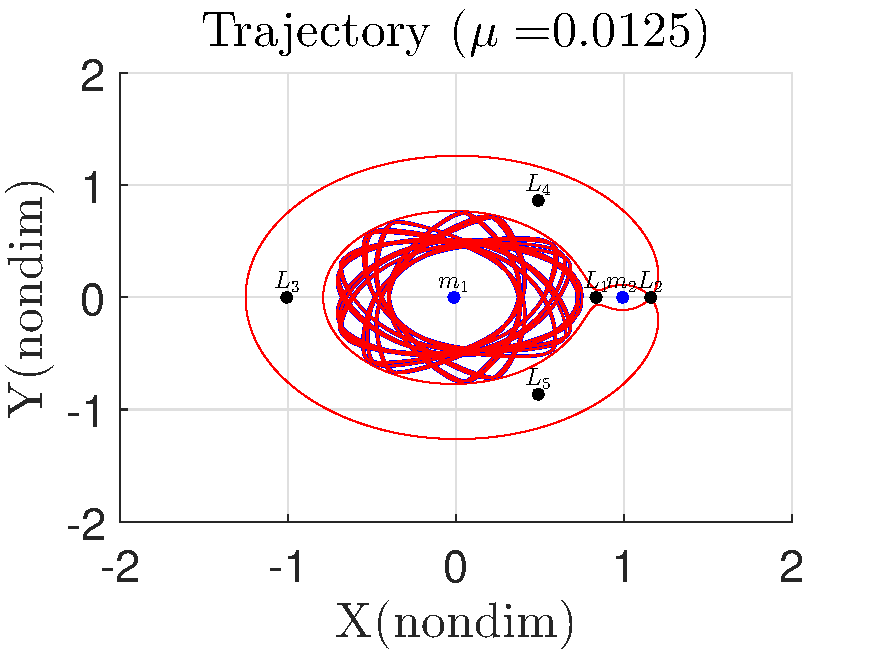
\includegraphics[width=\textwidth]{trajectory} 
                \caption{Earth-Moon three-body trajectory used for integrator comparision}
        \end{subfigure}~ %add desired spacing between images, e. g. ~, \quad, \qquad, \hfill etc. %(or a blank line to force the subfigure onto a new line) 
%       \begin{subfigure}[htbp]{0.3\textwidth} 
%               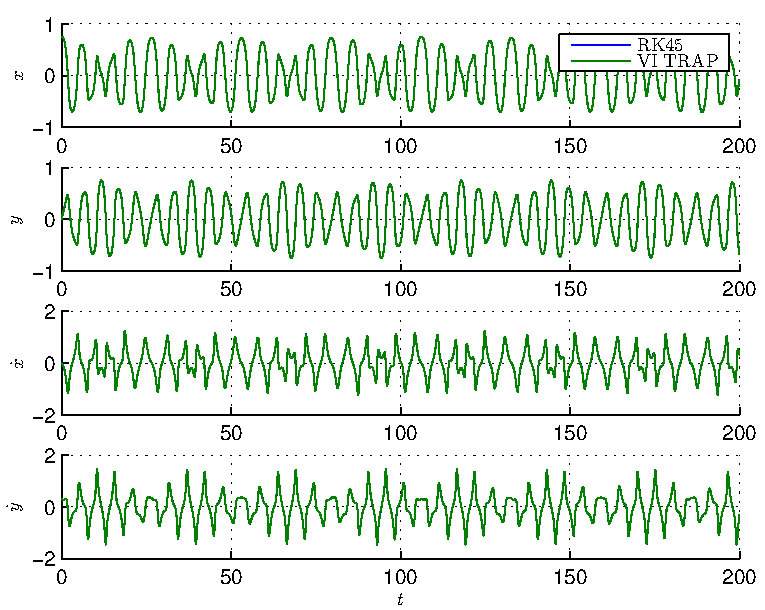
\includegraphics[width=\textwidth]{components} 
%               \caption{State \( \parenth{x , y, \dot{x}, \dot{y}}\)} \label{fig:compare_components} 
%       \end{subfigure} ~ %add desired spacing between images, e. g. ~, \quad, \qquad, \hfill etc. %(or a blank line to force the subfigure onto a new line) 
        \begin{subfigure}[htbp]{0.5\textwidth} 
                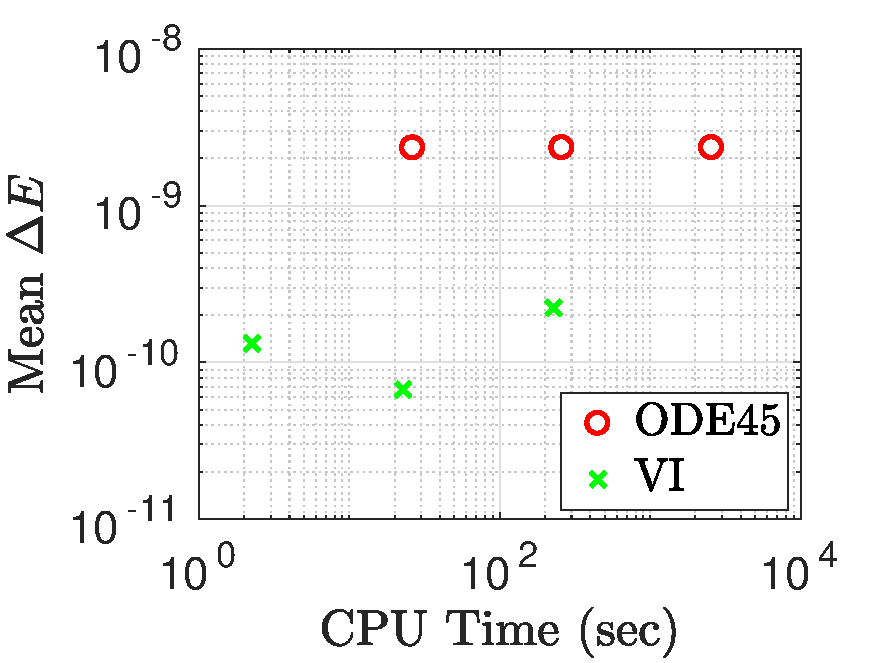
\includegraphics[width=\textwidth]{figures/cputimevsE.pdf} 
                \caption{Mean Jacobi integral deviation between variational integrator and Matlab \texttt{ODE45}} 
        \end{subfigure} 
        \caption{Integrator Comparison}
\end{figure}
A simulation comparing the variational integrator to a conventional Runge-Kutta method is given in~\cref{fig:integrator_compare}.
A particle is simulated from an initial condition of \( \vecbf{x}_0 = \begin{bmatrix} 0.75 & 0 & 0 & 0.2883\end{bmatrix}^T \) for \( t_f = 200 \approx 15\) years in the Earth-Moon system.
    The variational integrator uses a range of step sizes between \SIrange{4.72}{472}{\second} while the Runge-Kutta method uses a variable step size implemented via \texttt{ODE45} in Matlab.
    The step size of the variable integrator is varied to approximately match the run time required by the conventional \texttt{ODE45} integrator.
\Cref{fig:compare_trajectory} shows the trajectory of the spacecraft in the rotating reference for this comparison.
Both integration schemes result in trajectories that are initially nearly identical.
\Cref{fig:compare_energy} shows the mean Jacobi integral deviation over the entire simulation time as a function of computation time.
For a given computational effort, in the form of simulation run time, the variational integrator will provide a smaller energy deviation as compared to the convential integration scheme.
Over long simulation horizons or with the addition of small control inputs the inability of conventional integration schemes to accurately track the system energy limits the applicability of conventional techniques in which energy conservation is mandatory for characterizing the solution space.
\end{correction}
\item 
    \begin{itshape}
It may also be generally worth acknowledging the benefits of Taylor's method within the context of variational integrators:
Schmitt, J., Shingel, T., Leok, M., "LAGRANGIAN AND HAMILTONIAN TAYLOR VARIATIONAL INTEGRATORS," eprint arXiv:1703.06599, 2017

Online copy: https://arxiv.org/pdf/1703.06599.pdf 
\end{itshape}

This manuscript is not really focused on variational integrators but rather the design of transfer trajectories using reachability sets.
Interested readers can find a wide variety of literature on the relative benefits of all manner of variational integrators in papers focused on that topic specifically.

\item 
    \begin{itshape}
"Over long simulation horizons or with the addition of small control inputs this poor energy behavior limits the applicability of conventional techniques".  I think you need to add "in which energy conservation is mandatory for characterizing the solution space."
\end{itshape}

The additional clarification has been added to the manuscript and copied below.
\begin{correction}

Over long simulation horizons or with the addition of small control inputs the inability of conventional integration schemes to accurately track the system energy limits the applicability of conventional techniques in which energy conservation is mandatory for characterizing the solution space.
\end{correction}

\item 
    \begin{itshape}
Section 5 - This method, while very useful in its given context is highly dependent on the use of the PCRTB in the framework of the current analysis.  This needs to somehow be conveyed.  3D transfers are significantly more challenging when it comes to exploiting Poincare sections.  It can be done, but more subplots, dimensions, and data storing are necessary to view the subspace - save to say, it is a more challenging endeavor that must be acknowledged for general purpose low-thrust mission design.
\end{itshape}

An additional paragraph has been added to the beginning of the section which discusses our reachability based transfer approach.
This additional content is copied below.

\begin{correction}
The numerical examples presented in this section are designed in the context of the PCRTBP.
The dynamic environment has a four dimensional state space and offers a convient integration constant in the form of the Jacobi integral.
As a result, there are well defined methods to define and exploit \Poincare sections, which result in straightforward two-dimensional subspaces of the system.
Our approach uses the \Poincare section to approximate the reachability set on this reduced subspace.
As a result, this approach is more difficult to apply to three-dimensional transfers in the general three body problem.
\Poincare sections in the case of the general six dimensional state space are significantly more challenging and typically require more complicated visualization techniques. 
However, this is an area of active research and some of the authors future research is aimed at implementing this approach for non-planar transfer trajectories.
\end{correction}

\item
    \begin{itshape}
Figures 10D and 13D - the authors need to present these plots in dimensional coordinates so that they may be reconciled with what existing technology can produce.  I recommend Newtons or milliNewtons.  For example, the NEXT (NASA evolutionary xenon thruster) can produce 0.25 Newtons of thrust at maximum power (~7 kW).  The XR5 Hall thruster can produce comparable thrust at 4.5 kW of power.  These are currently the highest-power single engines other than the ARM Hall thruster which is not flight ready yet.  For these examples to be reconciled against the capability of existing technology, we need to see the required forces that are being demanded from the optimal control problem.  It may be that the results are beyond the scope of current technology - that's fine - just say that they are examples and that it's ongoing work to formulate example problems that capture existing technology better.
\end{itshape}

The mentioned plots of the control input have been modified to show the data in dimensional units (Newtons). 
Some additional detail has been provided in the manuscript which discusses the choice of \( u = 0.75 \) and it's realtionship to the current state of the art thruster systems.
The modified plots are not included here but the additional content is copied below in response to a different but related comment.

\item
    \begin{itshape}
"The multiple shooting method is implemented in this paper which alleviates many of the issues associated with single shooting approaches."  Did the authors attempt single shooting for their example problems before coming to this conclusion?  With proper scaling, and problem formulation, there are examples in the literature of single shooting yielding robust results.  

Example: 
Ranieri, C. and Ocampo,C..  "Indirect Optimization of Spiral Trajectories", Journal of Guidance, Control, and Dynamics, Vol. 29, No. 6 (2006), pp. 1360-1366.

So, justification for its selection may be warranted.  You could always find a reference in which this trade space was really explored thoroughly to show why you made the choice.
\end{itshape}

Our original attempt at solving the optimal control problem did rely on single shooting.
However, during our investigation it was found that it was quite difficult for solutions to converge.
As a result, we decided to implement the multiple shooting approach in hopes of generating more consistent and robust solutions.
While it is possible to use single shooting, such as the provided reference, it is known that the single shooting approach will have greater sensitivity to initial costate errors as compared to a multiple shooting method.
This can be alleviated, or entirely mitigated in the case of~\cite{ranieri2006}, it is highly case specific and dependent on a large variety of case specific techniques. 
For example, the work in~\cite{ozimek2010a} used both a single shooting and multiple shooting approach to solve the optimal control problem.
The large sensitivity of the single shooting approach was mitigated through the use of the multiple shooting method, at the expense of additional design variables.

In the manuscript, additional detail has been added in this section which describes the difficulties of the single shooting approach and our decision to use the multiple shooting method.
The modified portion of the manuscript is copied here.
\begin{correction}
Rather than numerical integration over the entire time interval, multiple shooting segments the interval into several smaller sub-arcs~\cite{stoer2013}.
This multiple shooting approach incorporates additional interior constraints but reduces the sensitivity of the costates along each sub-arc.
The use of the multiple shooting method reduces the sensitivity of changes in the initial costate at the expense of additional design variables, but has been shown to provide more stable and robust solutions~\cite{ozimek2010a}.
\end{correction}

\item
    \begin{itshape}
"In this work, we use the Matlab nonlinear solver fsolve to solve the system of nonlinear equations defined by the multiple shooting algorithm."  Can authors give some additional details?  Which fsolve algorithm? trust region dogleg,  trust region, or Levenberg-Marquardt?  Which additional options?  E.g. various tolerances.  For users of this method it's also useful to see the iteration history (more comments on this later).
\end{itshape}

Additional detail has been incorporated which discusses the specific solver used in computing the solutions. 
The description does not specifically mention all of the possible options in \texttt{fsolve} but rather gives the key components used in our solution.
This approach seems to be consistent with the literature, e.g.~\cite{ozimek2010a,stuart2010}.
The modified portion is copied below.

\begin{correction}
In this work, we use the Matlab nonlinear solver \texttt{fsolve} to solve the system of nonlinear equations defined by the multiple shooting algorithm.
Within \texttt{fsolve}, we use the trust-region dogleg solver which makes use of the Powell dogleg procedure for computing a step direction and magnitude to minimize successive iterations of the solver.
All numerical integration is performed using the discrete variational integrator described in~\cref{sec:discrete_var}.
\end{correction}

\item
    \begin{itshape}
Did the authors experiment with the number of multiple shooting stages in their example problems?  There must be some sort of "sweet spot" in number of stages for the example problems attempted.  If I missed it, I apologize, but I didn't see it.
\end{itshape}

We did spend considerable time in determining the appropriate number of stages. 
One key issue was that our implementation in software depended on dividing the total number of integration steps by the number of interior stages.
For simplicity, this reduced to possible number of stages to an even number. 
Additionally, we discovered that adding many stages tended to degrade the solution and cause difficulties in covergence. 
The solver would tend to ensure a continuous trajectory, by satisfying the interior stages, at the expense of the terminal stage. 
Some additional detail has been provided that mentions our choice of the number of stages and has been copied below.

\begin{correction}
Based on experimentation, we use four stages in our multiple shooting method.
This provided the best performance and convergence stability while minimizing the difficulties in additional interior constraints.
\end{correction}


\item 
    \begin{itshape}
Section 6.1 - I don't think you need to explain how you created the three-body orbits.  This can be found in many references - You can just cite a reference and give the orbit specifications.  (Starting with line 49, page 18, up to line 21 page 19.)
\end{itshape}

The discussion of generating periodic orbits in the three body problem has been removed.
It replaced with a small introduction mentioning the differential correction process and a citation to a relevant resource. 
The revised paragraph is copied below.

\begin{correction}
The first objective is to design a transfer trajectory from a planar periodic orbit about the \( L_1\) Lagrange point to a bounded orbit in the vicinity of the Moon.
The target region is created by choosing an initial condition of \( x_0 = \begin{bmatrix}1.05 & 0 & 0 & 0.35 \end{bmatrix}^T \) with \( \mu = 0.0125 \).
The target set is propagated over a period of \( t = \num{20} \) in non-dimensional units which corresponds to approximately \num{1.5} years.
\Cref{fig:moon_orbit} shows that the target set remains in the vicinity of the Moon, or \( m_2\), in the rotating reference frame. 
This type of orbit would be useful for a variety of mission scenarios.
The bounded trajectories of the vehicles and constant line of sight to both the Moon and the Earth would allow for constant communication for future manned missions and potential habitats.
The initial set is a planar periodic orbit about \( L_1\), which is generated using the process of differential correction of a linear approximation~\cite{koon2011}.
\end{correction}

\item
    \begin{itshape}
"We define a maximum magnitude of the thrust as umax = 0.75 and assume we can point the thrust in any direction within the plane." And  "we again assume a upper bound on the thrust magnitude of umax = 0.75."  What was the reason behind this? Isn't this a pretty large value of dimensional acceleration for your problem of interest?  Even if it's chosen for demonstrative purposes, there should be some sort of explanation as to why.  In the context of what electric propulsion systems can deliver, it could be arguable that this value isn't really "low-thrust" but "finite-thrust".
\end{itshape}

The maximum thrust magnitude was chosen to be approximately \SI{1}{\newton} for an assumed \SI{500}{\kilo\gram} spacecraft. 
While larger than the NEXT thruster mentioned earlier, a cluster of similar engines could provide the required thrust (assuming adequate available power). 
Additional detail has been included in the manuscript describing this thrust limit in dimensional units. 
\begin{correction}
Next, we determine the reachability set with the addition of a low thrust control input.
We define a maximum magnitude of the thrust as \( u_{max} = 0.75 \) and assume we can point the thrust in any direction within the plane. 
This model is representative of many spacecraft which have a body fixed thruster and attitude control system.
We assume a fully actuated spacecraft model which decouples the translational and rotational dynamics.
This acceleration limit is approximately \( u_{max} = \SI{2}{\milli\meter\per\second\squared} \) in the Earth-Moon system.
Assuming a fixed spacecraft mass of \SI{500}{\kilo\gram}, this model defines a maximum thrust of \SI{1}{\newton}.
Currently, the NASA NEXT xenon thruster is able to provide approximately \SI{0.25}{\newton} of thrust, and a cluster of such engines could be used to provide the desired thrust used in this work~\cite{schmidt2008}.
The trajectories are generated from a fixed initial state of \( \vecbf{x}_0 = \begin{bmatrix}0.8156 & 0 & 0 & 0.1922 \end{bmatrix}^T \) over a fixed time span of \( t_f = 1.4 \).
This initial state lies on the initial periodic orbit and the time of flight is equivalent to one half period of the initial periodic orbit. 
\end{correction}

\item 
    \begin{itshape}
Is this method exceptionally difficult to adapt to create a numerical example from LEO or GTO?  These would be the most pragmatically interesting departure orbits to the mission design community.  Section 6.2 presents an example from GEO, but it is unlikely that GEO represents a "typical" parking orbit, since there is no reason to insert a spacecraft into GEO before it transfers to the destination orbit.  This should be called out in the conclusions or future work.
\end{itshape}

This method is not difficult to adapt for other scenarios.
However, there is a certain amount of experimentation to ensure that trajectories converge. 
In addition, the details in this paper were designed in the context of the planar three body problem and as a result and extension to the nonplanar GTO is non trivial.
The examples presented are primarily aimed at introducing and demonstrating the feasibility of this approach, rather than designing operational mission profiles for spacecraft.
However, this is a valuable comment and a goal of future research. 
Additional detail has been included in the conclusion discussing this topic.

\item 
    \begin{itshape}
The authors should discuss some statistics of the convergence of their multiple shooting TPBVP - number of iterations, compute time, etc.
\end{itshape}

Most of the literature tends to not spend time discussing the low level details of the computational procedure, e.g.~\cite{grebow2011,stuart2010}.
In addition, the number of iterations, computation time and even the eventual cost function value are highly dependent on the specific system and more specifically the implementation of the algorithm in software. 
There are a wide variety of works which are focused more exclusively on the computational implementation of various optimal control techniques which do spend significant time on the computational characteristics.
However, our manuscript is primarily focused on demonstrating the feasbility of using reachability sets to design transfer trajectories.
As a result, there is not much benefit to detailed statistics of the implementation of this methodology.

\item 
    \begin{itshape}
Can any intuition be gained from reporting the optimal converged cost function values in section 6.1 and 6.2?  One could at least compare them to compare the reachability in the two different examples.
\end{itshape}

The cost function only parameterizes the distance between the controlled and uncontrolled terminal states on the \Poincare section. 
In addition, each state which lies on the reachable set would typically have a different distance and therefore a different coverged cost function value. 
Furthermore, it would be difficult to characterize a single parameter which characterizes the reachable set, in the form of the cost function, for all states of the reachable set. 
Also, the cost function is highly dependent on the transit time of trajectory, i.e. a longer transit time corresponds to a larger reachable set and a larger magnitude of the cost function.
However, this is an interesting suggestions for future research.
For example, the cost function gives some indication of area/volume of the reachable set. 
It may be possible to use this value as another way to characterize the subspace on the \Poincare section and is an intriguing avenue of future research.

\item
    \begin{itshape}
"Low energy transfers from the Earth to the Lagrange points are necessary for future missions."  One must be careful not to confuse these with traditional "low-energy transfers" to the moon, which use Sun third-body perturbations to transfer into lunar orbit.  These are what many mission designers define as "low-energy" lunar transfers.  This is actually a four-body problem (Sun, Earth, moon, spacecraft), and represents additional delta-V savings (as was done with NASA's GRAIL mission.)

Example:


Parker, J. and Anderson, R., "Low-Energy Lunar Trajectory Design," DEEP SPACE COMMUNICATIONS AND NAVIGATION SERIES, Jet Propulsion Laboratory Pasadena, California, July 2013.

Online Copy: https://descanso.jpl.nasa.gov/monograph/series12/LunarTraj--Overall.pdf
\end{itshape}
This sentence has been modified to make it more clear that we're discussing low thrust propulsion rather than low-energy transfers.
The modified sentence is copied below.

\begin{correction}
Transfers from the Earth to the Lagrange points, through the use of low-thrust electric propulsion, offer an additional and potentially shorter time of flight in comparison to the low-energy transfers which utilize solar perturbations.
\end{correction}

\item 
    \begin{itshape}
For what it's worth, exploiting sun perturbations with low-thrust in the Earth-moon RTBP would be highly beneficial and represent a worthy avenue of future research (more on this below.)
\end{itshape}

This is a very useful and interesting suggestion and something that we will take into consideration for future research.

\item 
    \begin{itshape}
The conclusions of the paper should acknowledge other potentially limiting factors of the presented analysis

-Omits advantage of exploiting fourth body perturbation (Sun in Earth/moon RTBP)

-Transfers are 2D only, method is more challenging to adapt to 3D

-Presented control magnitudes are dimensionally large, and more work is needed to determine feasibility of approach for lower accelerations

-Thrust and mass are completely decoupled from the analysis, which is limiting in terms of finding suitable hardware that can deliver the controls needed, as currently presented.
\end{itshape}

The conclusion has been expanded with some discussion of the drawbacks of this research and avenues of future work.
The modified conclusion is copied below.

\begin{correction}
In this paper, an optimal transfer process which combines concepts of reachability and \Poincare section is used to generate transfer between planar periodic orbits in the three-body problem.
The \Poincare section allows for trajectory design on a lower dimensional phase space and simplifies the process.
The indirect optimal control formulation enables straightforward method of incorporating additional path and control constraints.
However, the use of optimal control techniques leads to open loop trajectories that are not robust to model uncertainties or disturbances.
Furthermore, our approach relies heaviliy on the relative simplicity of the PCRTBP and this method is much more challenging for the non-planar case.

There is additional research to extend these results to more general transfer scenarios in future work.
The incorporation of fourth body perturbations, such as the Sun in the Earth-Moon system, offers an additional method of increasing the reachable set with the combined use of the solar perturbation and low-thrust propulsion.
In addition, the assumed acceleration magnitude is currently beyond the capabilities of current electric propulsion systems.
Furthermore, this analysis did not consider the effect of variable mass on the optimal control solution.
This will result in a more complicated optimal control problem and is a focus of future research.
Finally, Lyapunov control theory, which has previously been applied to the two-body problem, is being investigated in the hope of designing closed loop control schemes for this three-body scenario~\cite{chang2002}.
The addition of attitude dynamics and realistic pointing constraints would significantly improve the applicability of this work.
\end{correction}
\end{enumerate}
\section*{Reviewer 2}


Reviewer \#2: PAPER SUMMARY:
The contribution of the authors is the synthesis of reachability theory with traditional low-energy mission design approaches to ease the study of the low-thrust mission design space in the CR3BP.  A crucial point is that reachability analysis in non-integrable systems is typically limited by the dimensionality of the control parameterization, which can be extremely large for continuous-thrust problems, depending on the time discretization used.  The authors numerically probe the boundaries of the reachable space by optimizing a distance metric on the Poincare section, avoiding the extreme cost of unmotivated exploration.  Numerical experiments show how the method could be applied in two CR3BP orbit transfer scenarios.  For a multi-rev solution, the method is applied once per rev and the reachable end state with minimal distance to the target manifold is used as the basis for the next rev.


ASSESSMENT:
The central premise of the paper - using optimization of Poincare distance as a guiding motivation to make low-thrust reachability analysis more tractable - is interesting, useful, and to my knowledge reasonably novel.  Furthermore, the quality of the writing is good (at local scales) and there is an appropriate degree of literature review.  However, there are two major problems with this paper.

First, in terms of composition, large portions of the paper are spent on lengthy development of foundational work that is well-known within the astrodynamics community and available in textbooks. Secondly, the contributions and findings of the authors feel highly preliminary and do not seem to evaluate their method at significant depth.

While there are the beginnings of a good article within this manuscript, it is not sufficiently close to publishable form to be accepted.  I recommend that the paper be rejected and that the authors push their investigation a bit further.  The eventual publication should focus less on background and should provide more insight into the fundamental properties of their method, using more rigorously constructed and analyzed examples.

I can sympathize that there was quite a long road to get to the point of understanding this topic and generating results in it. I hope that the authors will not find this verdict too discouraging, as I believe that stronger results are well within their reach.


SPECIFIC FEEDBACK:
\begin{itemize}
    \item
    \begin{itshape}
*** Bloat
In the introduction, the exposition of the problem could be considerably condensed, given the venue of publication. Additionally, the somewhat sprawling discussion jumps back and forth, and many key points seem to be repeated more than necessary.  It needs to be organized into titled subsections with specific scope.
\end{itshape}

The introduction is reduced and many of the paragraphs have been reworded and combined. 
In addition, the extended discussion of the benefits of variational integrators is removeda.
In the interest of space/clarity the modified introduction is not copied here.

The development of the CR3BP, invariant manifolds and Poincare maps, all go on a bit too long. These should be refreshers to the audience that expose the specific equations and concepts that you'll be leveraging, not full-on introductions to well-established areas.  Spending several pages on variational principles is way too much.

Section 4 ends on page 14 with essentially a thesis statement ("In this paper, we...").  Strive to push the boundary between background and new developments to a much earlier point in the paper; it shouldn't happen so late that you need to remind the audience what the paper is for.

A missing relevant reference: "On target for Venus — set oriented computation of energy efficient low thrust trajectories" (Dellnitz, Junge, Post, and Thiere, 2006)

*** Variational Integrators
Many of the specific claims regarding the use of a variational integrator are unsubstantiated and, I believe, incorrect. Why is energy drift "even more detrimental" with regards to "the long term effects of low-thrust"?  I would need to be convinced that a non-geometric integrator's energy drift relative to a constant energy baseline is significantly different from its drift relative to a gradually shifting baseline corresponding to low thrust. The specific claims about the numerical stability of derivatives also don't seem related to energy preservation.  

Apart from these claims, I question the need for a variational integrator in the first place. The example in section 3.4 is not convincing because there is no apples-to-apples basis for the comparison; a variable-step integrator with unspecified tolerance is compared to a fixed-step integrator with an arbitrary step size.  Integrator comparisons should consider error in proportion to compute cost, which can be tuned by step size or tolerance.  Also, fixed step seems inappropriate for a path through diverse dynamic regimes, and it's not clear that the problem scope calls specifically for energy preservation (especially since the idea is to use low thrust to mitigate some time cost of exploiting the problem structure).  

*** Figures
Altogether, the figures need more descriptive captions.  

Figure 4 does not show what I think you intend it to show; it looks like two periodic circular orbits.

Figure 6 is also very unclear.  Is phi supposed to be \texttt{theta\_d}?  Is the bounding curve specifically circular, or should it be a more general shape?

Consider plotting the intersections of manifolds with the Poincare section as continuous curves.  

Also consider zooming/scaling as necessary to show the details you discuss.

*** Method/Examples
I urge a revisiting of the claims with regards to optimality.  The optimization method is being initialized with *something*, and stationary points are *local* extrema.  More precise claims and assurances about solution quality (and therefore the validity of the computed reachable set boundary) are needed.  

How damaging is the assumption of a fixed travel time?  And how about the specification of a specific departure point on the initial orbit?

In Fig 10b, it is hard to see, but appears that the low-thrust-reachable set is actually *centered* on part of the target set.  Is this related to the existence of the uncontrolled transfer opportunity?  There must be some more clear way to show how the low thrust set expands upon the zero thrust set.  Perhaps beginning with the time horizon of the zero-thrust opportunity, and successively lowering it, would help.  

Perhaps there is also a better way to show what the control is doing, e.g., in some alternative parametrization?  This could help provide assurances that the solution is doing something meaningful and is not just stuck in a weird local minimum.  

In the second example, what do you lose by chaining together multiple reachability-based steps?  Aren't you imposing that the trajectory routinely returns to the energy level of the Poincare section? How feasible would it be to conduct a single reachability analysis covering multiple revolutions? And can you use knowledge about directionality of movement on the Poincare section to limit the scope of your reachability search?

In general, please devote more depth to probing the strengths, weaknesses, and fundamental properties of the method.  Considering extreme cases can help with this.
\end{itemize}
\bibliography{library}
\bibliographystyle{spmpsci}
\end{document}

